%%%%%%%%%%%%%%%%%%%%%%%%%%%%%%%%%%%%%%%%%
% Jacobs Landscape Poster
% LaTeX Template
% Version 1.0 (29/03/13)
%
% Created by:
% Computational Physics and Biophysics Group, Jacobs University
% https://teamwork.jacobs-university.de:8443/confluence/display/CoPandBiG/LaTeX+Poster
% 
% Further modified by:
% Nathaniel Johnston (nathaniel@njohnston.ca)
%
% This template has been downloaded from:
% http://www.LaTeXTemplates.com
%
% License:
% CC BY-NC-SA 3.0 (http://creativecommons.org/licenses/by-nc-sa/3.0/)
%
%%%%%%%%%%%%%%%%%%%%%%%%%%%%%%%%%%%%%%%%%

%----------------------------------------------------------------------------------------
%	PACKAGES AND OTHER DOCUMENT CONFIGURATIONS
%----------------------------------------------------------------------------------------

\documentclass[final]{beamer}
\usepackage{xcolor}

\usepackage{tikz}
\usetikzlibrary{positioning,graphs,arrows,calc,shapes,petri,backgrounds,fit}
\usepackage[scale=1.24]{beamerposter} % Use the beamerposter package for laying out the poster

\usetheme{confposter} % Use the confposter theme supplied with this template
\setbeamercolor{block title}{fg=cmured,bg=white} % Colors of the block titles
\setbeamercolor{block body}{fg=black,bg=white} % Colors of the body of blocks
\setbeamercolor{block alerted title}{fg=white,bg=cmured} % Colors of the highlighted block titles
\setbeamercolor{block alerted body}{fg=black,bg=black!1} % Colors of the body of highlighted blocks
\setbeamercolor{title in headline}{fg=cmured!90!black,bg=white}
\setbeamercolor{cboxb}{fg=black,bg=cmured!80!black}
% Many more colors are available for use in beamerthemeconfposter.sty

%-----------------------------------------------------------
% Define the column widths and overall poster size
% To set effective sepwid, onecolwid and twocolwid values, first choose how many columns you want and how much separation you want between columns
% In this template, the separation width chosen is 0.024 of the paper width and a 4-column layout
% onecolwid should therefore be (1-(# of columns+1)*sepwid)/# of columns e.g. (1-(4+1)*0.024)/4 = 0.22
% Set twocolwid to be (2*onecolwid)+sepwid = 0.464
% Set threecolwid to be (3*onecolwid)+2*sepwid = 0.708

\newlength{\sepwid}
\newlength{\onecolwid}
\newlength{\twocolwid}
\newlength{\threecolwid}
\setlength{\paperwidth}{48in} % A0 width: 46.8in
\setlength{\paperheight}{36in} % A0 height: 33.1in
\setlength{\sepwid}{0.024\paperwidth} % Separation width (white space) between columns
\setlength{\onecolwid}{0.22\paperwidth} % Width of one column
\setlength{\twocolwid}{0.464\paperwidth} % Width of two columns
\setlength{\threecolwid}{0.708\paperwidth} % Width of three columns
\setlength{\topmargin}{-0.5in} % Reduce the top margin size
%-----------------------------------------------------------

\usepackage{graphicx}  % Required for including images

\usepackage{booktabs} % Top and bottom rules for tables

\usepackage{listings}

\definecolor{codegreen}{rgb}{0,0.6,0}
\definecolor{codegray}{rgb}{0.5,0.5,0.5}
\definecolor{codepurple}{rgb}{0.58,0,0.82}
\definecolor{backcolour}{rgb}{0.95,0.95,0.92}
\lstdefinestyle{mystyle}{
    backgroundcolor=\color{backcolour},   
    commentstyle=\color{codegreen},
    keywordstyle=\color{magenta},
    numberstyle=\tiny\color{codegray},
    stringstyle=\color{codepurple},
    basicstyle=\ttfamily\scriptsize,
    breakatwhitespace=false,         
    breaklines=true,                 
    captionpos=b,                    
    keepspaces=true,                 
    numbers=left,                    
    numbersep=5pt,                  
    showspaces=false,                
    showstringspaces=false,
    showtabs=false,                  
    tabsize=2,
    postbreak={\space\space\space}
}
\lstdefinestyle{textstyle}{
	basicstyle=\ttfamily
}

% Add CMU logo and Scotty dog to template
\addtobeamertemplate{headline}{}{\begin{tikzpicture}
\useasboundingbox (0,0) rectangle (0,0);
\node (blah) at (0,0) {};
\node[inner sep=0pt] (CMU) at (-44.15in,2.1in) {
\includegraphics[height=3.7in]{cmu_large_transparent.png}};
\node[inner sep=0pt] (scotty) at (-1.5in,2.1in) {
\includegraphics[height=3.7in]{scotty}};
\end{tikzpicture}}

%----------------------------------------------------------------------------------------
%	TITLE SECTION 
%----------------------------------------------------------------------------------------

\title{Automatic Refactoring of Robotics Code} % Poster title

\author{Audrey Seo\footnotemark[1], Ian Voysey\footnotemark[2], Ruben Martins\footnotemark[2]} % Author(s)

\institute{\footnotemark[1]Wellesley College; \footnotemark[2]School of Computer Science, Carnegie Mellon University} % Institution(s)

%----------------------------------------------------------------------------------------

\begin{document}



\addtobeamertemplate{block end}{}{\vspace*{2ex}} % White space under blocks
\addtobeamertemplate{block alerted end}{}{\vspace*{2ex}} % White space under highlighted (alert) blocks

\setlength{\belowcaptionskip}{2ex} % White space under figures
\setlength\belowdisplayshortskip{2ex} % White space under equations

\begin{frame}[t] % The whole poster is enclosed in one beamer frame

\begin{columns}[t] % The whole poster consists of three major columns, the second of which is split into two columns twice - the [t] option aligns each column's content to the top

\begin{column}{\sepwid}\end{column} % Empty spacer column

\begin{column}{\onecolwid} % The first column

%----------------------------------------------------------------------------------------
%	Problem
%----------------------------------------------------------------------------------------

% ||||\\\  ||||\\\     /////\\   ||||\\\   ||       ||////// ||\      /||
% ||    \\ ||    \\   //     \\  ||    \\  ||       ||       ||\\    //||
% ||    // ||    //  ||       || ||    //  ||       ||       || \\  // ||
% ||||///  ||\\\\\   ||       || ||||\\\   ||       ||/////  ||  \\//  ||
% ||       ||    \\  ||       || ||    \\  ||       ||       ||        ||
% ||       ||     ||  \\     //  ||     \\ ||       ||       ||        ||
% ||       ||     ||   \\\\\//   ||/////// ||////// ||////// ||        ||

\begin{alertblock}{Problem}
\begin{itemize}
\item ROS is a framework for programming robots
\item First version, ROS1, incompatible with ROS2
\item Want to automatically upgrade ROS1 to ROS2
\end{itemize}

\end{alertblock}

%----------------------------------------------------------------------------------------
%	Motivation
%----------------------------------------------------------------------------------------


% ||\      /||   /////\\   ////////// || \\      //    //\\  ////////// ||   /////\\   ||\     ||
% ||\\    //||  //     \\      ||     || \\      //   //  \\     ||     ||  //     \\  ||\\    ||
% || \\  // || ||       ||     ||     || \\      //  //    \\    ||     || ||       || || \\   ||
% ||  \\//  || ||       ||     ||     || \\      // //======\\   ||     || ||       || ||  \\  ||
% ||        || ||       ||     ||     ||  \\    //  //      \\   ||     || ||       || ||   \\ ||
% ||        ||  \\     //      ||     ||   \\  //   //      \\   ||     ||  \\     //  ||    \\||
% ||        ||   \\\\\//       ||     ||    \\//    //      \\   ||     ||   \\\\\//   ||     \||

\begin{block}{Motivation}

\begin{itemize}
\item Difficult to update code (e.g. Python 2.7 vs 3)
\item ROS1 has major security vulnerabilities
\item Programming robots, which has real world applications and consequences, is higher priority than updating dependencies and refactoring code
\end{itemize}

\end{block}

%------------------------------------------------

\begin{figure}
\lstinputlisting[language=C++,style=mystyle]{ros1_listener.cpp}
\caption{Original C++ code for a ``listener'' node, using ROS1.}
\label{fig:listenercode}
\end{figure}

\begin{figure}
\lstinputlisting[language=C++,style=mystyle]{listener.sketch}

\caption{The sketch created from the code in Fig. \ref{fig:listenercode} by putting holes (denoted by \texttt{?\#?}) in the place of any ROS methods. The original ROS1 method is shown in the comments after each hole.}
\label{fig:listenersketch}
\end{figure}

%----------------------------------------------------------------------------------------

\end{column} % End of the first column

\begin{column}{\sepwid}\end{column} % Empty spacer column

\begin{column}{\twocolwid} % Begin a column which is two columns wide (column 2)

%\begin{columns}[t,totalwidth=\twocolwid] % Split up the two columns wide column
%\end{columns} % End of the split of column 2 - any content after this will now take up 2 columns width

%----------------------------------------------------------------------------------------
%	IMPORTANT RESULT
%----------------------------------------------------------------------------------------
\begin{figure}

\newlength{\nodelength}
\setlength{\nodelength}{2.8in}
%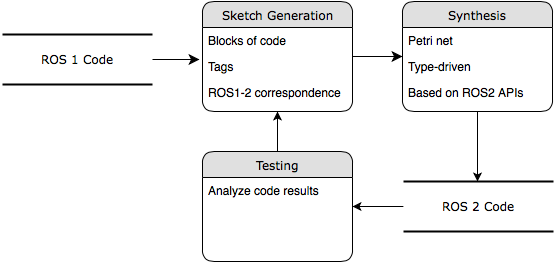
\includegraphics[width=\linewidth]{images/diagram}
\begin{tikzpicture}[node distance=1in,
					bend angle=45,
					every node/.style={rounded corners=10mm},
					code/.style={rectangle,fill=white,inner sep=0.2in,minimum size=\nodelength,minimum height=3in,font=\ttfamily,text width=\nodelength,align=center},
					phase/.style={rectangle,fill=white,minimum height=3in,minimum width=1.6\nodelength,text width=1.6\nodelength,align=center},
					myarrow/.style={->,>=stealth',line width=2.5mm}]
	\node[code] (ros1) at (0,0) {
\includegraphics[width=\nodelength]{roslogo}\\ ROS1 Code};
	\node[phase,right=of ros1] (sketch)		{
\includegraphics[width=.7\nodelength]{sketchpencil}\\Sketch Generation};
	\node[phase,above right=of sketch] (synth)		{Synthesis};
	\node[code,below right=of synth] (ros2)		{
\includegraphics[width=.8\nodelength]{ros2logo}\\ROS2 Code};
	\node[phase,below right=of sketch] (test)		{Testing};
	
	\draw[myarrow] (ros1) to (sketch);
	\draw[myarrow] (sketch) to[bend left] (synth);
	\draw[myarrow] (synth) to[bend left] (ros2);
	\draw[myarrow] (ros2) to[bend left] (test);
	\draw[myarrow] (test) to[bend left] (sketch);
	
	\begin{scope}[on background layer]
		\node[rounded corners=0mm,fill=backcolour,fit=(ros1) (ros2) (sketch) (synth) (test),inner sep=.5in] {};
	\end{scope}
\end{tikzpicture}


\end{figure}


%\begin{alertblock}{Important Result}
%
%Lorem ipsum dolor \textbf{sit amet}, consectetur adipiscing elit. Sed commodo molestie porta. Sed ultrices scelerisque sapien ac commodo. Donec ut volutpat elit.
%
%\end{alertblock} 

%----------------------------------------------------------------------------------------

\begin{columns}[t,totalwidth=\twocolwid] % Split up the two columns wide column again

\begin{column}{\onecolwid} % The first column within column 2 (column 2.1)

%----------------------------------------------------------------------------------------
%	SKETCH GENERATION
%----------------------------------------------------------------------------------------


%  //////  ||    // ||////// //////////  ///\\\   ||      || 
% //    \\ ||   //  ||           ||    //      \\ ||      || 
% \\\      ||  //   ||           ||   ||          ||      || 
%    \\\   || //    ||/////      ||   ||          ||======|| 
%       \\ ||  \\   ||           ||   ||          ||      || 
% \\    // ||   \\  ||           ||    \\      // ||      || 
%  //////  ||    \\ ||//////     ||      \\\///   ||      || 
%    ///\\\    ||////// ||\     || ||////// ||||\\\      //\\  ////////// ||    ///\\\    ||\     ||
%  //      \\  ||       ||\\    || ||       ||    \\    //  \\     ||     ||  //      \\  ||\\    ||
% ||           ||       || \\   || ||       ||    //   //    \\    ||     || ||        || || \\   ||
% ||           ||/////  ||  \\  || ||/////  ||\\\\\   //======\\   ||     || ||        || ||  \\  ||
% ||    ////// ||       ||   \\ || ||       ||    \\  //      \\   ||     || ||        || ||   \\ ||
%  \\      //  ||       ||    \\|| ||       ||     || //      \\   ||     ||  \\      //  ||    \\||
%    \\\///    ||////// ||     \|| ||////// ||     || //      \\   ||     ||    \\\///    ||     \||

\begin{block}{Sketch Generation}
A \textbf{sketch} is a partially defined program with all ROS1 code removed (see Fig. \ref{fig:listenersketch}). We had to create these manually, but in the future, this could be automatically generated using data flow analysis. %In this first prototype, we have manually divided up the code into blocks.

% Note: there *appears* to be 17 different tags, but two of the tags are actually just the same exact thing: message and messages lol
All ROS2 methods were \textbf{tagged} with 16 different keys that encoded programmer intent (see Table \ref{tab:tags}).

As first test cases for synthesis, we chose two node programs: a ``listener'' and a ``talker'' that communicate over a channel called a \textit{topic}, a core part of the ROS framework. The talker sends messages, which the listener receives.
\end{block}

%As first test cases for refactoring, we chose two node programs: a ``listener'' and a ``talker'' that communicate over a channel called a \textit{topic}. Though just two programs might seem like a small sample size, the topic model drives the entirety of interactions in ROS, so this actually more representative of other ROS code samples than it would seem.

\begin{table}[h]
	\footnotesize
	\begin{tabular}{llllllll}
						&\multicolumn{6}{c}{Overlap with}	\\
		Tag				&\texttt{other}	&\textt{sub}	&\texttt{pub}	&\texttt{constructor}	&\texttt{ros}	&\texttt{node}	&	Total	\\
		\texttt{node}	&0				&4				&4				&14						&0						&-				&66	\\
		\texttt{ros}	&0				&3				&0				&6						&-						&-				&41	\\
	\texttt{constructor}&7				&9				&6				&-						&-						&-				&31	\\
		\texttt{pub}	&7				&0				&-				&-						&-						&-				&16	\\
		\texttt{sub}	&0				&-				&-				&-						&-						&-				&16	\\
		\texttt{other}	&-				&-				&-				&-						&-						&-				&37
	\end{tabular}
	\caption{Breakdown of the top 5 tags, and all others are in the ``other'' category. The average number of tags per method was 1.5, thus the numbers in the total column don't add up to the number of methods in the search space: 142.}
	\label{tab:tags}
\end{table}




%----------------------------------------------------------------------------------------

\end{column} % End of column 2.1

\begin{column}{\onecolwid} % The second column within column 2 (column 2.2)

%----------------------------------------------------------------------------------------
%	SYTHESIS
%----------------------------------------------------------------------------------------

%  ////// \\      // ||\     || ////////// ||      || ||////// //////  ||  //////
% //    \\ \\    //  ||\\    ||     ||     ||      || ||      //    \\ || //    \\
% \\\       \\  //   || \\   ||     ||     ||      || ||      \\\      || \\\
%    \\\     \\//    ||  \\  ||     ||     ||======|| ||/////    \\\   ||    \\\
%       \\    ||     ||   \\ ||     ||     ||      || ||            \\ ||       \\
% \\    //    ||     ||    \\||     ||     ||      || ||      \\    // || \\    //
%  //////     ||     ||     \||     ||     ||      || ||////// //////  ||  //////



\begin{figure}
\def\myscale{0.8}

\begin{tikzpicture}[scale=\myscale,
					every node/.style={scale=\myscale},
					trans/.style={transition,font=\ttfamily\footnotesize,minimum width=1cm,minimum height=3cm,fill=black},
					every label/.style={font=\ttfamily\footnotesize},
					flow/.style={->,>=stealth',thick,line width=1mm},
					myinput/.style={text width=9in,align=center,font=\ttfamily\footnotesize}]

\node[place,label=left:{std::string},tokens=2] 												(stdstring) {};
\node[trans,label=above left:{Node::make\_shared},above right=1.2in of stdstring] 			(makeshared) {};
\node[place,label=above:{shared\_ptr<Node>},right=1.2in of makeshared] 						(ptrnode) {};
\node[trans,label=right:{->},below right=1.2in of ptrnode] 									(derefnode) {};
\node[place,label=right:{Node}] at ($(derefnode.south)-(0.7in,1.2in)$) 						(n) {};
\path let \p1=($(stdstring)!($(makeshared)!.5!(ptrnode)$)!(derefnode)$) in
	coordinate (middle) at (\p1);
%\node[place,label=right:{size\_t}] at ($(stdstring)!($(makeshared)!.5!(ptrnode)$)!(derefnode)$)	(sizet) {};
\node[place,label=above:{size\_t},tokens=1] at ($(stdstring)!(makeshared)!(derefnode)$)	(sizet) {};
\node[place,label=above:{callback},tokens=1] at ($(stdstring)!(ptrnode)!(derefnode)$) (callback) {};


\node[myinput,above=3.5in of middle]			(inputs)	{apis: [[Node::make\_shared], [create\_subscription]]\\types: \{std::string: 2,\\size\_t: 1, callback: 1\}};

\path let \n1={-1.2in},
		  \p1=($(inputs.south)+(0,\n1)$) in
		 coordinate (myinputarrowend) at (\p1);

\node[trans,label=below left:{create\_subscription(A)}] at ($($(n)-(5,0)$)!($(makeshared)!.5!(ptrnode)$)!(n)$)	(createsubA) {};
\node[place,label=above right:{shared\_ptr<Subscription>},below=1in of createsubA] 			(ptrsub) {};
\path let \n1={-1.5in},
		  \p1=($(ptrsub) + (0,\n1)$),
		  \p2=($(ptrsub) + (2,\n1)$) in
	coordinate (derefsubA) at (\p1)
	coordinate (derefsubB) at (\p2);
\node[trans,label=right:{->}] at ($(derefsubA)!(derefnode)!(derefsubB)$) 	(derefsub) {};
\node[place,label=below right:{Subscription}] at ($($(derefsub.south)+(-2in,-1.2in)$)!(n)!($(derefsub.south)+(2in,-1.2in)$)$)				(sub) {};
\draw let \p1=(stdstring),\p2=(derefsub) in
		(\x1,\y2) node (ptrmsgplace) {};
\node[place,label=above:{shared\_ptr<msg::String>}] at  (ptrmsgplace) (ptrmsg) {};
\node[trans,label=below:{publish},below=1.8in of ptrsub] 	(publish) {};

\node[myinput,below=1.4in of publish,align=left] (output) {shared\_ptr<Node> n = Node::make\_shared(node\_name);\\n->create\_subscription(topic\_name,chatterCallback,queue\_size);};
\path let \n1={1.2in},
		  \p1=($(output.north)+(0,\n1)$) in
		  coordinate (myoutputarrowbegin) at (\p1);

\draw[flow] (stdstring) to [bend left=45] 				(makeshared);
\draw[flow] (makeshared) to 							(ptrnode);
\draw[flow] (stdstring) to [bend right=35] 				(createsubA);
\draw[flow] (ptrnode) 	to [bend left=45]				(derefnode);
\draw[flow] (sizet) to [bend right=40]									(createsubA);
\draw[flow] (callback) to [bend left=40]				(createsubA);
\draw[flow] (derefnode) to [bend left=20]				(n);
\draw[flow] (n) to 										(createsubA);
\draw[flow] (createsubA) to 							(ptrsub);
\draw[flow] (ptrmsg) to [bend right=45]					(publish);
\draw[flow] (ptrsub) to [bend left=20]					(derefsub);
\draw[flow] (derefsub) to [bend left=10]				(sub);
\draw[flow] (sub) to [bend left=10]						(publish);

\draw[->,line width=5mm,draw=cmured,fill=cmured] (inputs) to (myinputarrowend);
\draw[->,line width=5mm,draw=cmured,fill=cmured] (myoutputarrowbegin) to (output);

\end{tikzpicture}

\caption{Partial petri net of ROS2 methods for the listener example (see Fig. \ref{fig:listenercode}). Input and output for synthesis is shown above and below, respectively.}
\label{fig:petri}
\end{figure}



%\begin{tikzpicture}[transition/.style={rectangle,draw=black,fill=black,text=white,minimum width=2mm,font=\ttfamily\footnotesize},
%					place/.style={draw=black,minimum width=2cm,font=\ttfamily\footnotesize},
%					small place/.style={place,circle},
%					big place/.style={place,ellipse, minimum height=3cm},
%					flow/.style={->,>=stealth',thick}]
%\node[transition] (makeshared) at (0,0) {Node::make\_shared};
%\node[small place] (stdstring) at ($(makeshared)+(2,3in)$)	{std::string};
%\node[big place] (2 and 3) (node) at ($(makeshared)+(0,-3in)$) {std::shared\_ptr<Node>};
%\node[transition] (createsub) at ($(node)+(3in,-3in)$) {Node::create\_subscription};
%\draw[flow] (stdstring) -- (makeshared);
%\end{tikzpicture}

%----------------------------------------------------------------------------------------

\end{column} % End of column 2.2

\end{columns} % End of the split of column 2

\end{column} % End of the second column

\begin{column}{\sepwid}\end{column} % Empty spacer column

\begin{column}{\onecolwid} % The third column

\begin{block}{Synthesis}
The ROS2 code synthesis is driven by searching a petri net (see Fig. \ref{fig:petri}), where the nodes are types and the transitions are ROS2 methods.

%However, in a petri net that has 308 places and 560 transitions, this problem is a lot more difficult than Fig. \ref{fig:petri} would make it appear.
\end{block}


%----------------------------------------------------------------------------------------
%	RESULTS
%----------------------------------------------------------------------------------------

% ||||\\\   ||//////  //////   ||    || ||    ////////  //////  
% ||    \\  ||       //    \\  ||    || ||       ||    //    \\ 
% ||    //  || 	     \\\       ||    || ||       ||    \\\ 
% ||\\\\\   ||/////     \\\	   ||    || ||       ||       \\\
% ||    \\  ||             \\  ||    || ||       ||          \\
% ||     || ||       \\    //  \\    // ||       ||    \\    //
% ||     || ||//////  //////    \\\///  ||////// ||     //////

\begin{figure}
\lstinputlisting[language=C++,style=mystyle]{listener_synthesized.cpp}

\caption{An example of a ``correct'' synthesized listener program, where ``correct'' means it should typecheck, compile, and communicate with the talker.}
\end{figure}

\begin{block}{Results}
The resulting petri net has 
\begin{itemize}
\item 308 places (types)
\item 560 transitions (ROS methods)
\end{itemize}

If we tried a naive approach to search the petri net, we would have at least $560^n$ solutions, where $n$ is the number of holes, or:
\begin{itemize}
\item $560^{4} \approx 9.83 \times 10^{10}$ listener candidates and
\item $560^{14} \approx 2.98 \times 10^{38}$ talker candidates.
\end{itemize}

Using tags and types to guide the search, we get:
\begin{itemize}
\item Listener: 16 candidate solutions
\item Talker: 64 candidate solutions.
\end{itemize}
\end{block}






%   ///\\\  ||      ||    //\\    ||       ||       ||////// ||\     ||   ///\\\   ||//////  //////
%  //    \\ ||      ||   //  \\   ||       ||       ||       ||\\    ||  //    \\  ||       //    \\
% ||        ||      ||  //    \\  ||       ||       ||       || \\   || ||         ||       \\\
% ||        ||======|| //======\\ ||       ||       ||/////  ||  \\  || ||         ||/////     \\\
% ||        ||      || //      \\ ||       ||       ||       ||   \\ || ||   ///// ||             \\
%  \\    // ||      || //      \\ ||       ||       ||       ||    \\||  \\    //  ||       \\    //
%   \\\///  ||      || //      \\ ||////// ||////// ||////// ||     \||   \\\///   ||//////  //////

\begin{block}{Challenges}
\begin{itemize}
\item C++ grammar: complicated and ambiguous
\item C++ types: parametric polymorphism
\item Diagnosing cause of failing test
\item Slow ROS compile time %$\to$ test cases not feasible
\end{itemize}

\end{block}


%----------------------------------------------------------------------------------------
%	CONTACT INFORMATION
%----------------------------------------------------------------------------------------

\setbeamercolor{block alerted title}{fg=black,bg=norange} % Change the alert block title colors
\setbeamercolor{block alerted body}{fg=black,bg=white} % Change the alert block body colors

%\begin{alertblock}{Contact Information}
%
%\begin{itemize}
%\item Web: \href{http://www.university.edu/smithlab}{http://www.university.edu/smithlab}
%\item Email: \href{mailto:john@smith.com}{john@smith.com}
%\item Phone: +1 (000) 111 1111
%\end{itemize}
%
%\end{alertblock}

%\begin{center}
%\begin{tabular}{ccc}
%
\includegraphics[width=0.4\linewidth]{logo.png} & \hfill & 
\includegraphics[width=0.4\linewidth]{logo.png}
%\end{tabular}
%\end{center}

%----------------------------------------------------------------------------------------

\end{column} % End of the third column

\end{columns} % End of all the columns in the poster

\end{frame} % End of the enclosing frame

\end{document}
